% Working manuscript for npj Computational Materials.
% The untouched Springer Nature template is retained as
% sn-article-template-original.tex.
\documentclass[pdflatex,sn-nature]{sn-jnl}

\usepackage{graphicx}
\usepackage{amsmath,amssymb,amsfonts}
\usepackage{xcolor}
\usepackage{booktabs}
\usepackage{multirow}
\usepackage{array}
\usepackage{url}

\newcommand{\placeholder}[1]{\par\smallskip\noindent{\color{orange!75!black}\textbf{PLACEHOLDER:} #1}\par\smallskip}
\newcommand{\claimboundary}[1]{\par\smallskip\noindent{\color{blue!65!black}\textbf{Claim boundary.} #1}\par\smallskip}
\newcommand{\kmc}{kMC}
\newcommand{\nleis}{NLEIS}

\raggedbottom

\begin{document}

\title[Formal countermodels for ion transport]{Formal countermodels expose when ion-transport predictions do not identify mechanism}

\author*[1]{\fnm{Yi} \sur{Cao}}
\affil*[1]{\orgname{Affiliation to be confirmed before submission}}

\abstract{Predictive agreement is often promoted to mechanistic evidence in ion-transport research, although different event networks, electrode allocations and ion-correlation structures can generate the same observable. Here we combine physics-guided hypothesis enumeration, certificate-derived formal obligations and numerical stress tests to make this ambiguity executable. In a fitted NASICON kinetic Monte Carlo model, a prospectively frozen 6,000-pass extension fails its study-level convergence and ordering gates; the only fully converged pair reverses the proposed conductivity ordering. Across 30 public paired linear and second-harmonic impedance spectra, joint fits pass a held-out error gate, whereas only 3 spectra meet a frozen electrode-allocation contraction criterion. A source-grounded polymer-electrolyte audit further shows that conductivity and segmental relaxation reject a composite scaling null without identifying whether diffusion, carrier population or collective correlations changed. These cases establish bounded forms of structural, practical and specification non-identifiability. They also define the observations required for closure. Formal proof certifies consequences of an encoded model; independent fidelity and empirical gates remain necessary before a mechanism can be assigned to a material.}

\keywords{mechanism identifiability, ion transport, formal verification, kinetic Monte Carlo, nonlinear impedance, polymer electrolyte, AI for science}

\maketitle

\begin{quote}
\textbf{Working-draft status (22 September 2026).} The NASICON and EIS/\nleis{} analyses reported below are complete under frozen contracts. The polymer negative-transference execution, independent theorem-to-claim fidelity reviews and material-level closure experiments are not complete. They are marked explicitly and are not included as positive results.
\end{quote}

\section{Introduction}

Accurate prediction and mechanistic identification answer different questions. A model may predict conductivity, an impedance spectrum or a relaxation trend while leaving several physical pathways compatible with the observation. This distinction becomes consequential when a scalar descriptor is interpreted as a transport mechanism, when a whole-cell signal is decomposed into electrode-specific contributions, or when a self-diffusion proxy is used to infer a collective transport coefficient. Artificial intelligence can expand the set of candidate explanations, but it can also produce an illusion of understanding if predictive success is treated as closure\cite{Krenn2022,Messeri2024}.

Materials studies in the Nature Portfolio illustrate the evidentiary standard required for a mechanistic claim. Large-scale NASICON simulations have been linked across local migration units, collective transport and matched electrochemical measurements\cite{Deng2022}; composition--conductivity design rules have been tested by combining first-principles calculation, text-mined data and synthesis\cite{WangNASICON2023}; and sequence-controlled polymer electrolytes have been argued from molecular design through ion environments to device behaviour\cite{Han2023}. In AI-enabled science, symbolic systems have recovered interpretable laws from observations\cite{Schmidt2009}, derivability from background axioms has discriminated formulae with similar data error\cite{Cornelio2023}, and closed-loop path sampling updates mechanistic models using the outcomes of new trajectories\cite{Jung2023}. These studies share a structure: the inference target is explicit, a second observable constrains the mechanism, and the limits of each evidence layer remain visible.

We ask a complementary question: what can be concluded when that closure is absent? We develop a workflow in which a natural-language claim is decomposed into assumptions, competing mechanisms, observables and a discriminating test. AI can propose and organize candidates, but a versioned scientific-claim certificate fixes their provenance and scope. Formal verification then checks whether the encoded conclusion follows from the encoded premises, while numerical and domain checks determine whether a countermodel is admissible. The final decision remains empirical.

We apply this workflow to three ion-transport settings. First, a NASICON \kmc{} study tests whether a mean local migration-barrier summary determines aggregate event kinetics or long-time transport. Second, a public linear EIS and second-harmonic \nleis{} dataset tests whether good held-out spectral prediction identifies a stable electrode allocation. Third, a polymer-electrolyte audit separates a directly observed conductivity--relaxation relation from electrode-polarization inversion and a packing-based causal narrative. The three cases represent structural, practical and specification non-identifiability, respectively. Our central result is deliberately bounded: formal countermodels and failed prospective gates can localize where mechanistic inference stops and specify what must be measured next. They do not, by themselves, select the mechanism operating in a material.

\section{Results}

\subsection{A certificate-mediated workflow separates logical validity from physical closure}

The workflow begins with historical evidence and physical knowledge, from which a mechanism library defines scientifically admissible candidates (Fig.~\ref{fig:workflow}). AI is used to enumerate competing explanations and construct a claim graph. Its output is converted into a certificate that records the natural-language claim, modality, scope, declared and hidden assumptions, competing mechanisms, observables, reference frame, evidence provenance, temporal cutoff and proposed closure observation. Formal obligations are derived from this certificate rather than from a pre-assigned label such as ``false mechanism''.

Three gates separate responsibilities. A semantic-fidelity review asks whether the formal theorem says what the scientific certificate says. A kernel or deterministic verifier checks the formal or numerical consequence. A domain and empirical review asks whether the witness is physically admissible and whether the material realizes it. Thus, Lean can prove that two encoded mechanisms are observation-equivalent or that a conjunction of premises implies an invariant. It cannot invent the physical mechanism, validate a measurement model or establish that the premises hold in the world.

\begin{figure*}[t]
\centering
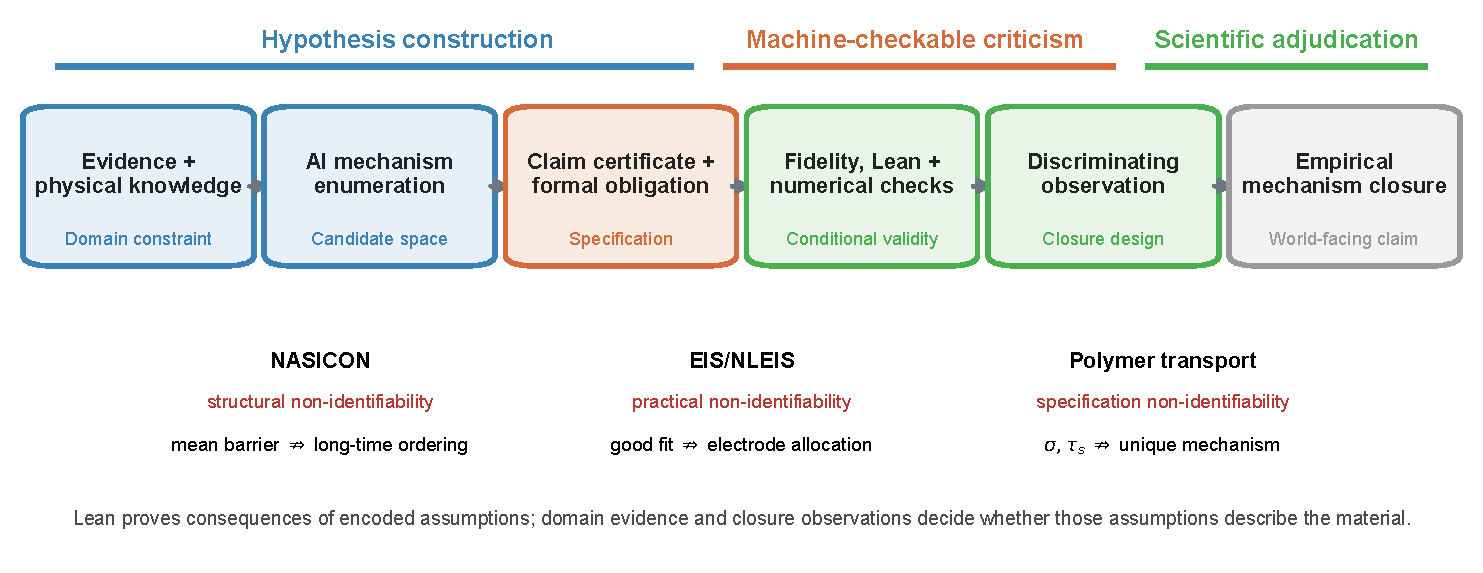
\includegraphics[width=0.98\textwidth]{figures/fig1_workflow.pdf}
\caption{\textbf{A certificate-mediated route from prediction to mechanism closure.} Historical evidence and a physics-based hypothesis library constrain AI-assisted enumeration of competing mechanisms. A versioned certificate fixes assumptions, scope, observables and the temporal cutoff before formalization. Independent fidelity review, Lean or deterministic verification and numerical/domain checks have distinct responsibilities. The output is a discriminating observation rather than an automatic claim that a mechanism is true. The three cases instantiate structural, practical and specification non-identifiability.}
\label{fig:workflow}
\end{figure*}

\subsection{Finite NASICON simulations do not establish a stable conductivity ordering}

Ion transport in NASICON is governed by a network of migration events whose rates depend exponentially on local barriers. Prior work used more than 2,000 ab initio-based \kmc{} simulations and experimental impedance to connect composition, spatial hopping and conductivity\cite{Deng2022}. A separate literature-scale study combined computation, synthesis and text-mined conductivity data to obtain composition-dependent design principles\cite{WangNASICON2023}. Against this background, our narrower question is whether matched structures with similar mean barriers inherit a stable aggregate kinetic or transport ordering inside one pinned fitted model.

The held-out initializer audit identified two structures that remain close under the declared mean-barrier summaries but differ in their aggregate initial hopping rates. A formal tolerance obligation checks the bounded statement that closeness of a scalar mean does not force equality of the aggregated exponential rate. This result is structural: it concerns the information discarded by the summary, not experimental pellet conductivity.

We then ran a prospectively frozen paired \kmc{} study at three seeds and extended each of the six trajectories to 6,000 passes (Fig.~\ref{fig:nasicon}). All requested runs completed. Four of six individual runs, and only one of three pairs, met the declared convergence criterion. The study-level convergence gate therefore failed. The directional-confirmation rule also failed: the paired conductivity ratios were 0.766, 1.094 and 0.604. In the only pair for which both trajectories passed the primary convergence gate, the structure with the larger initial aggregate rate had a lower late-window median conductivity (ratio 0.604).

This is a failure-preserving result. It does not warrant choosing a more favourable seed or redefining the convergence rule after seeing the data. It shows that the proposed promotion from initial-rate ordering to stable long-time conductivity ordering is not established under the frozen protocol, and it supplies a bounded ordering counterexample within the pinned fitted model.

\claimboundary{The result does not validate the fitted energy landscape, identify a physical transport mechanism, establish population-level generality or predict experimental pellet conductivity.}

\begin{figure*}[t]
\centering
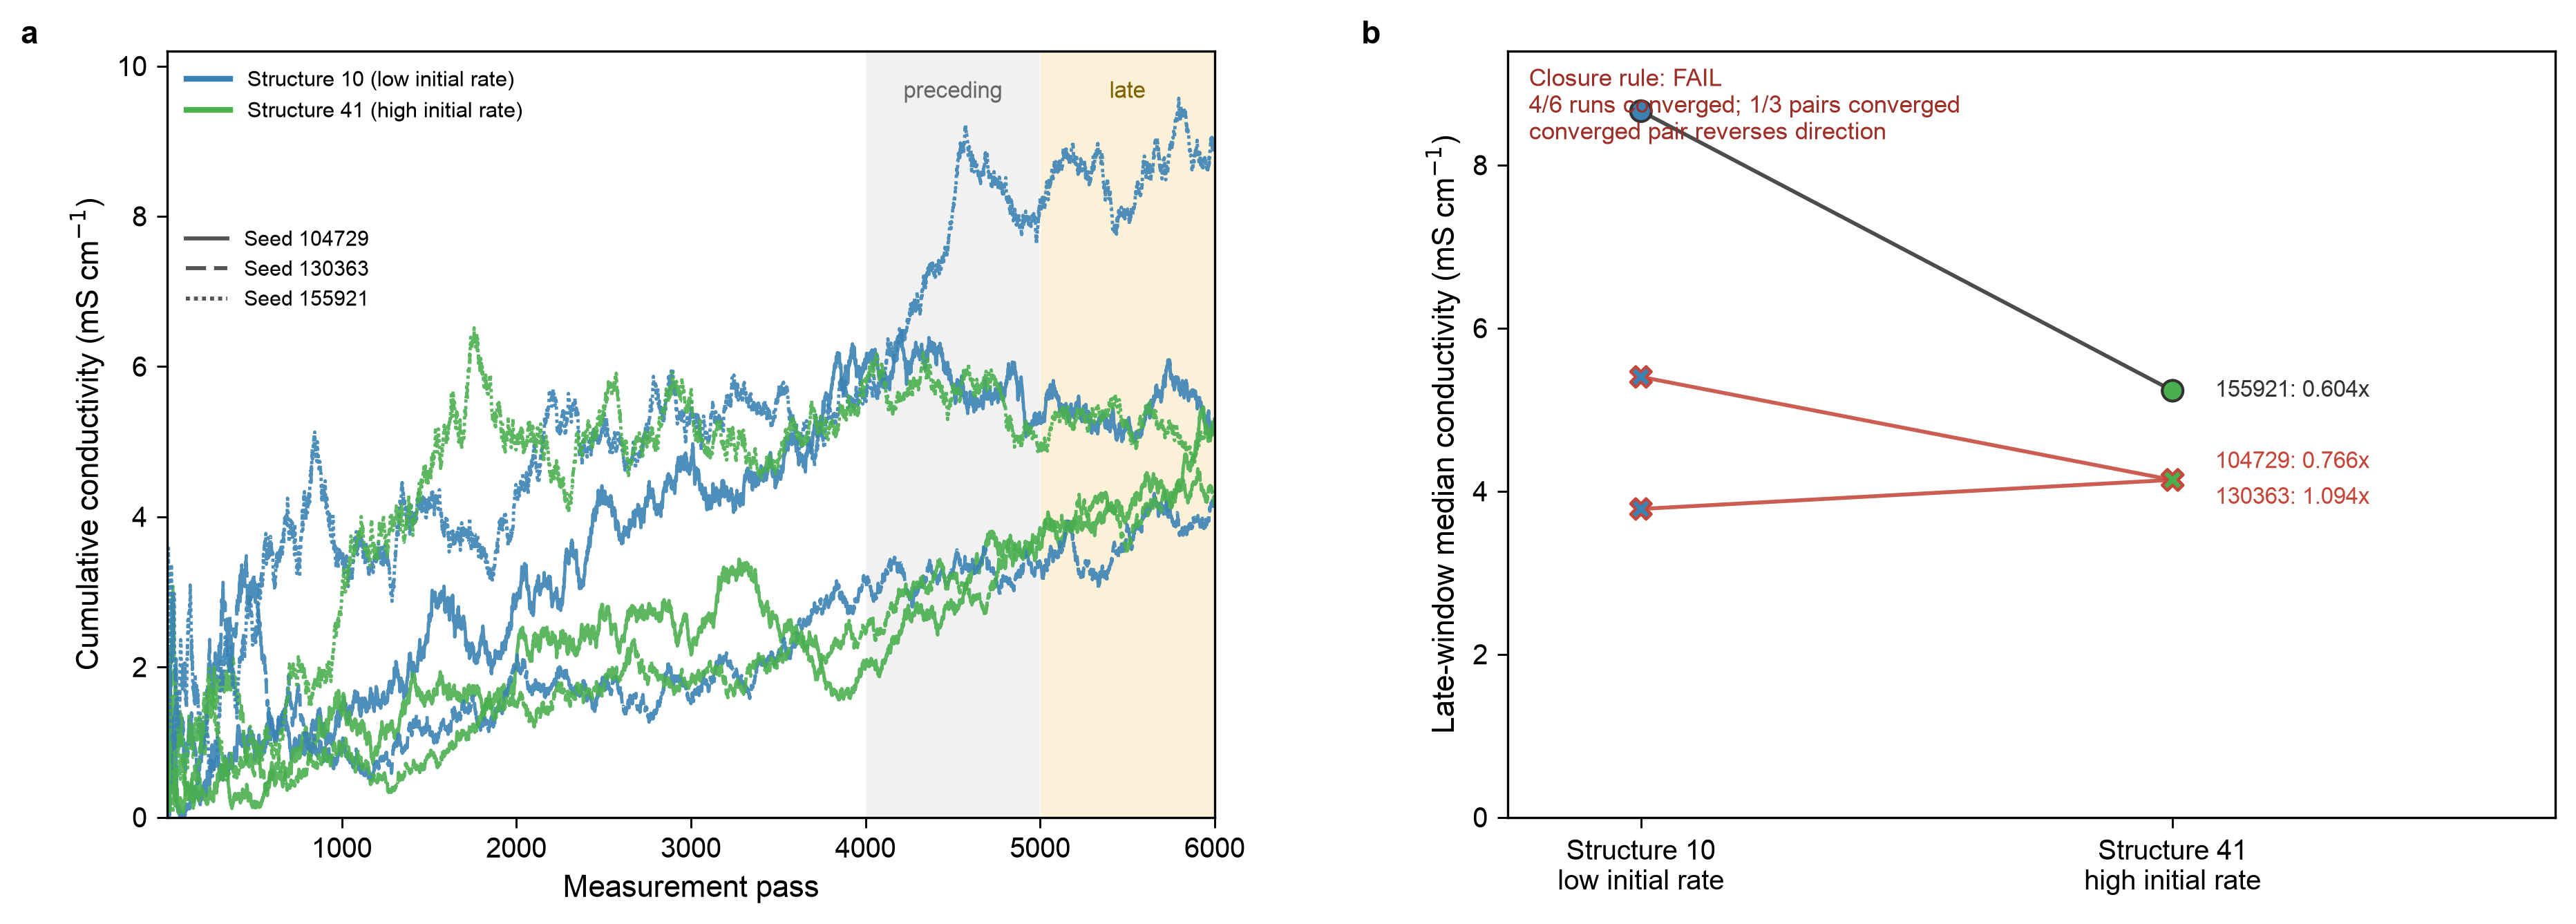
\includegraphics[width=0.94\textwidth]{figures/fig2_nasicon_extended_kmc.png}
\caption{\textbf{The extended NASICON \kmc{} study fails its promotion gates.} \textbf{a,} Convergence diagnostics for six 6,000-pass trajectories. Four individual runs and one complete pair pass the frozen criterion; the study-level convergence gate fails. \textbf{b,} Paired late-window median conductivities. The proposed directional rule is not reproduced across seeds, and the sole fully converged pair (seed 155921) reverses the initial-rate ordering (ratio 0.604). Values apply only to the pinned fitted \kmc{} model and protocol.}
\label{fig:nasicon}
\end{figure*}

\placeholder{Promote this case beyond a within-model counterexample only after preregistered longer trajectories and independent seeds pass convergence, event-network occupancy/correlation diagnostics identify a stable mediator, and matched-temperature impedance measurements on composition- and structure-matched samples agree within declared uncertainty.}

\subsection{Joint EIS/\nleis{} prediction does not guarantee practical electrode allocation}

For a two-electrode cell, a linear full-cell EIS signal can be represented schematically as the sum of positive- and negative-electrode contributions, whereas the second-harmonic signal has opposite parity and contains their difference\cite{Ji2023a,Ji2024b}. The elementary formal countermodel is immediate: allocations $(3,1)$ and $(2,2)$ have the same linear sum but different second-harmonic differences. The scientific question is not whether the second channel contains information in principle, but whether adding it contracts the practical allocation uncertainty under a frozen model, finite noise and multistart fitting.

We audited all 30 paired public spectra spanning state of charge, cell age and replicate. For each spectrum, identical held-out frequencies and multistart seeds were used for EIS-only and joint EIS/\nleis{} fits within a pinned two-electrode circuit family. Twenty-six spectra satisfied the preregistered eligibility rule. The joint fits passed the held-out error gate, with median EIS and \nleis{} normalized root-mean-square errors of 0.024 and 0.116, respectively (Fig.~\ref{fig:nleis}). However, only 3 of 30 spectra passed the frozen allocation-range contraction threshold. The joint confirmation rule therefore failed even though predictive adequacy passed.

This separation is scientifically informative. A low-error joint fit can coexist with weak practical identification of the target allocation. Conversely, the failed contraction rule does not show that \nleis{} is uninformative: the conclusion is conditional on the selected circuit family, parameterization, noise model, multistart design and contraction threshold.

\claimboundary{The result rejects only the frozen fixed-circuit practical-identifiability confirmation rule. It does not establish universal EIS non-identifiability, validate the circuit as the physical cell mechanism or identify solid-electrolyte transport causality.}

\begin{figure*}[t]
\centering
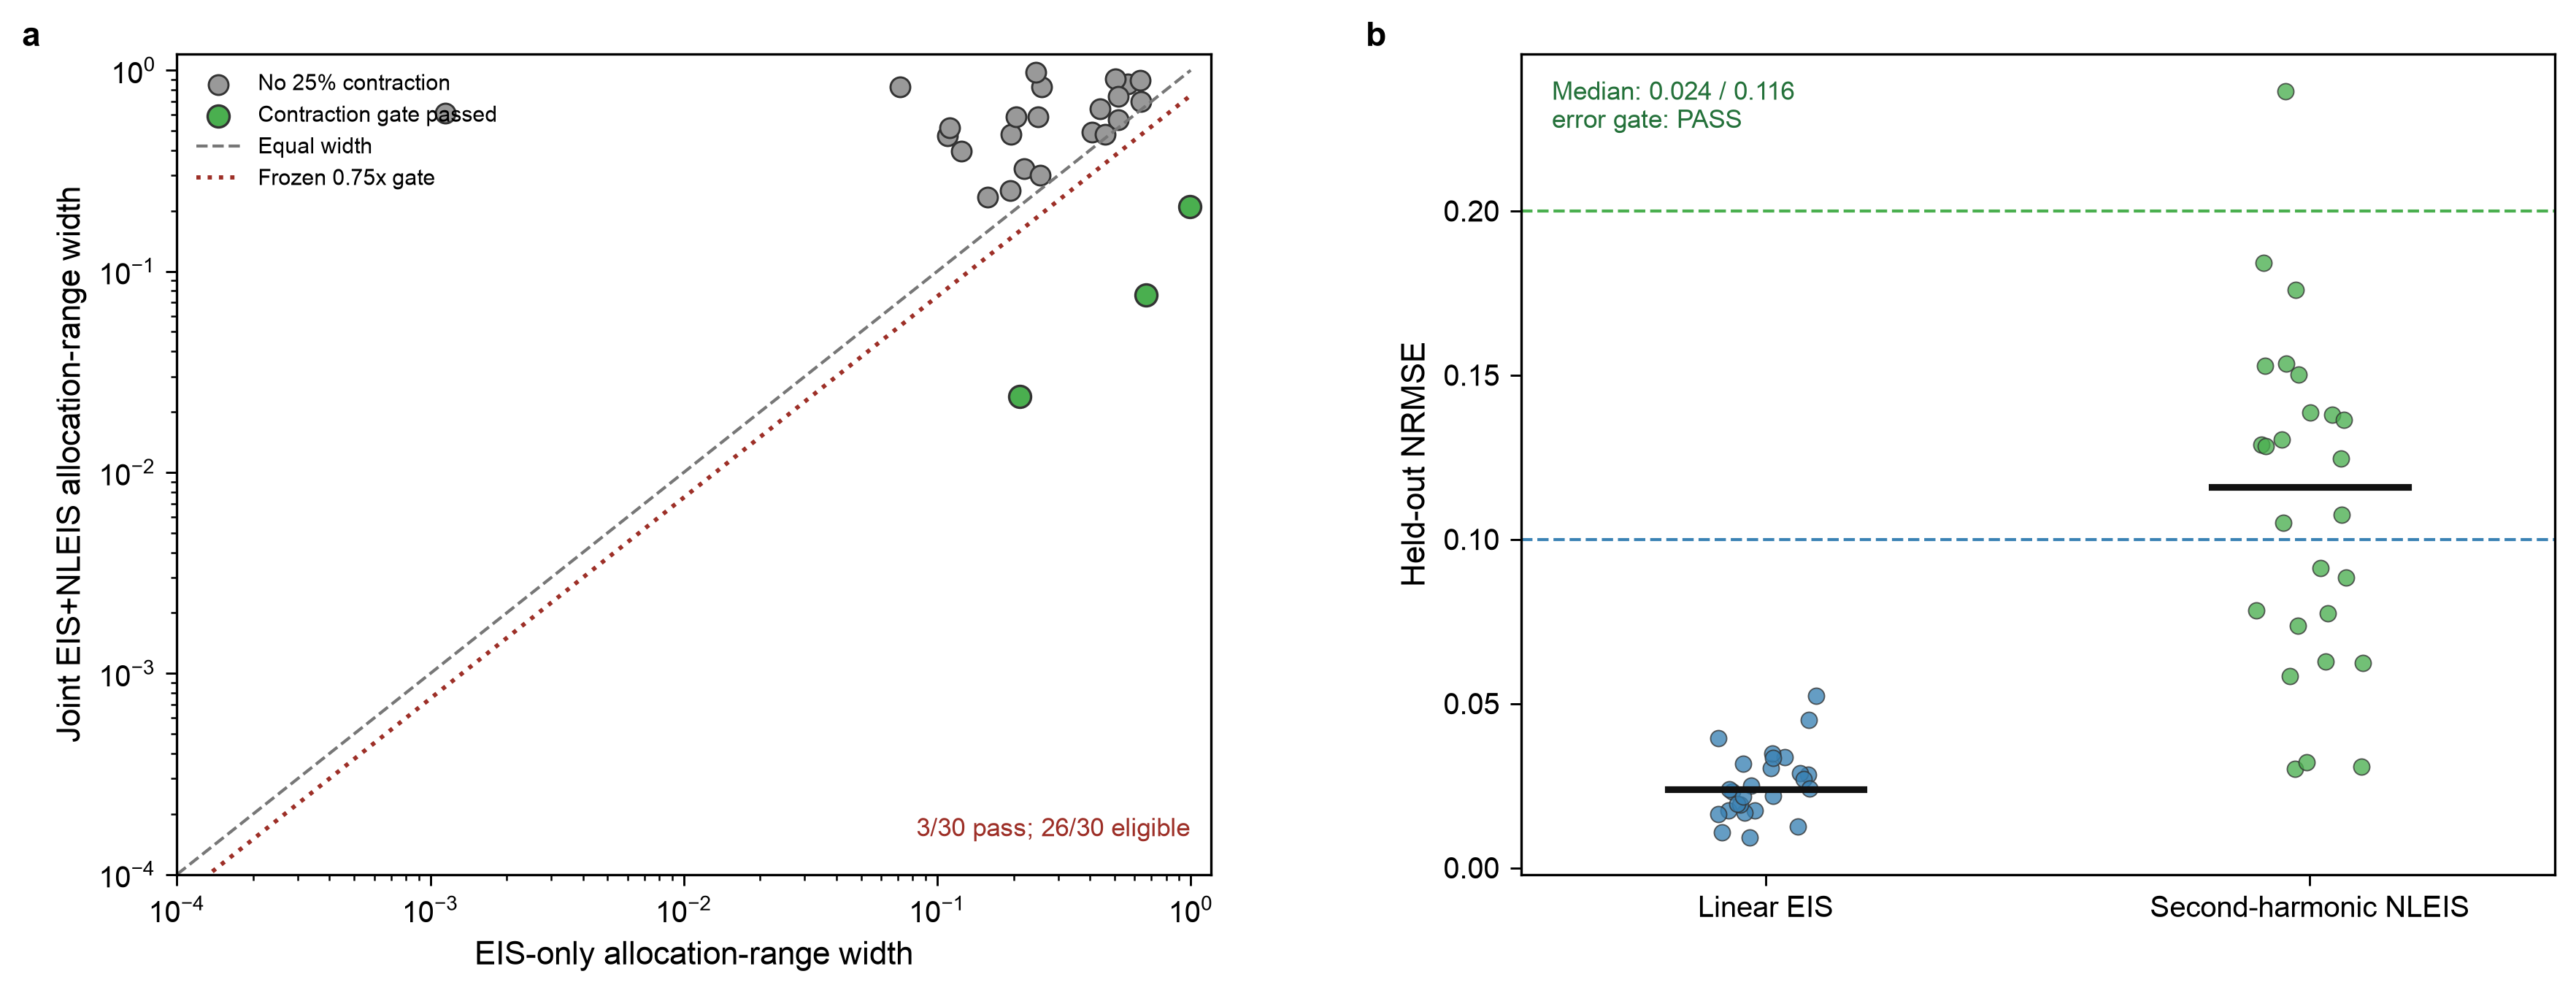
\includegraphics[width=0.94\textwidth]{figures/fig3_nleis_joint_fit.png}
\caption{\textbf{Predictive adequacy and practical allocation identifiability separate in the impedance study.} \textbf{a,} Electrode-allocation range under EIS-only and joint EIS/\nleis{} multistart fits for the eligible spectra. Only 3 of 30 spectra meet the frozen contraction rule. \textbf{b,} Held-out error remains low enough to pass the declared error gate (median EIS NRMSE 0.024; median second-harmonic \nleis{} NRMSE 0.116 among 26 eligible spectra). The combination demonstrates that prediction error alone does not certify parameter allocation.}
\label{fig:nleis}
\end{figure*}

\placeholder{Test circuit-family and uncertainty robustness using preregistered alternative mechanistic models, calibrated likelihoods and posterior predictive checks. Establish physical electrode attribution using half-cell/reference-electrode constraints or independently measured electrode parameters.}

\subsection{A polymer-electrolyte audit separates observation, inversion and mechanism}

Wang et al. reported fractional decoupling between ionic conductivity $\sigma$ and segmental relaxation time $\tau_s$ in five comb-like polymer electrolytes and related the trend to packing frustration in rigid polymers\cite{Wang2012}. A precise fully coupled null is not merely $\sigma\propto\tau_s^{-1}$. If
\begin{equation}
 \sigma(T)=\frac{q^2}{k_{\mathrm B}T}p(T)H(T)D(T),
\end{equation}
where $p$ is the effective carrier population and $H$ is a collective correlation factor, then the conjunction
\begin{equation}
 D(T)\tau_s(T)=C,\qquad p(T)=p_0,\qquad H(T)=H_0
\end{equation}
predicts the invariant
\begin{equation}
 \sigma(T)T\tau_s(T)=A,
\end{equation}
or a slope of $-1$ for $\log[\sigma(T)T]$ against $\log\tau_s(T)$.

The published exponents and multi-decade changes in $\sigma T\tau_s$ support rejection of this composite null in the named rigid-backbone materials. They do not identify which member of the conjunction fails. A temperature-dependent carrier population, changing distinct-ion correlations or a parallel local transport channel can generate the same observed deviation while $D\tau_s$ remains constant. Formal proofs check both the conditional invariant and an explicit carrier-variation countermodel.

The further decomposition of the dielectric response into diffusivity and mobile-ion fraction is model-mediated (Fig.~\ref{fig:polymer}). It depends on a Debye-like electrode-polarization model, an equal-cation/anion-diffusivity approximation, electrode assumptions and empirical normalization. Conditional agreement of two inversion formulae does not validate these shared physical premises. Likewise, packing frustration is compatible with the observations but is not uniquely selected over changes in carrier population, local hopping, ion clusters, collective correlations or morphology.

\begin{figure*}[t]
\centering
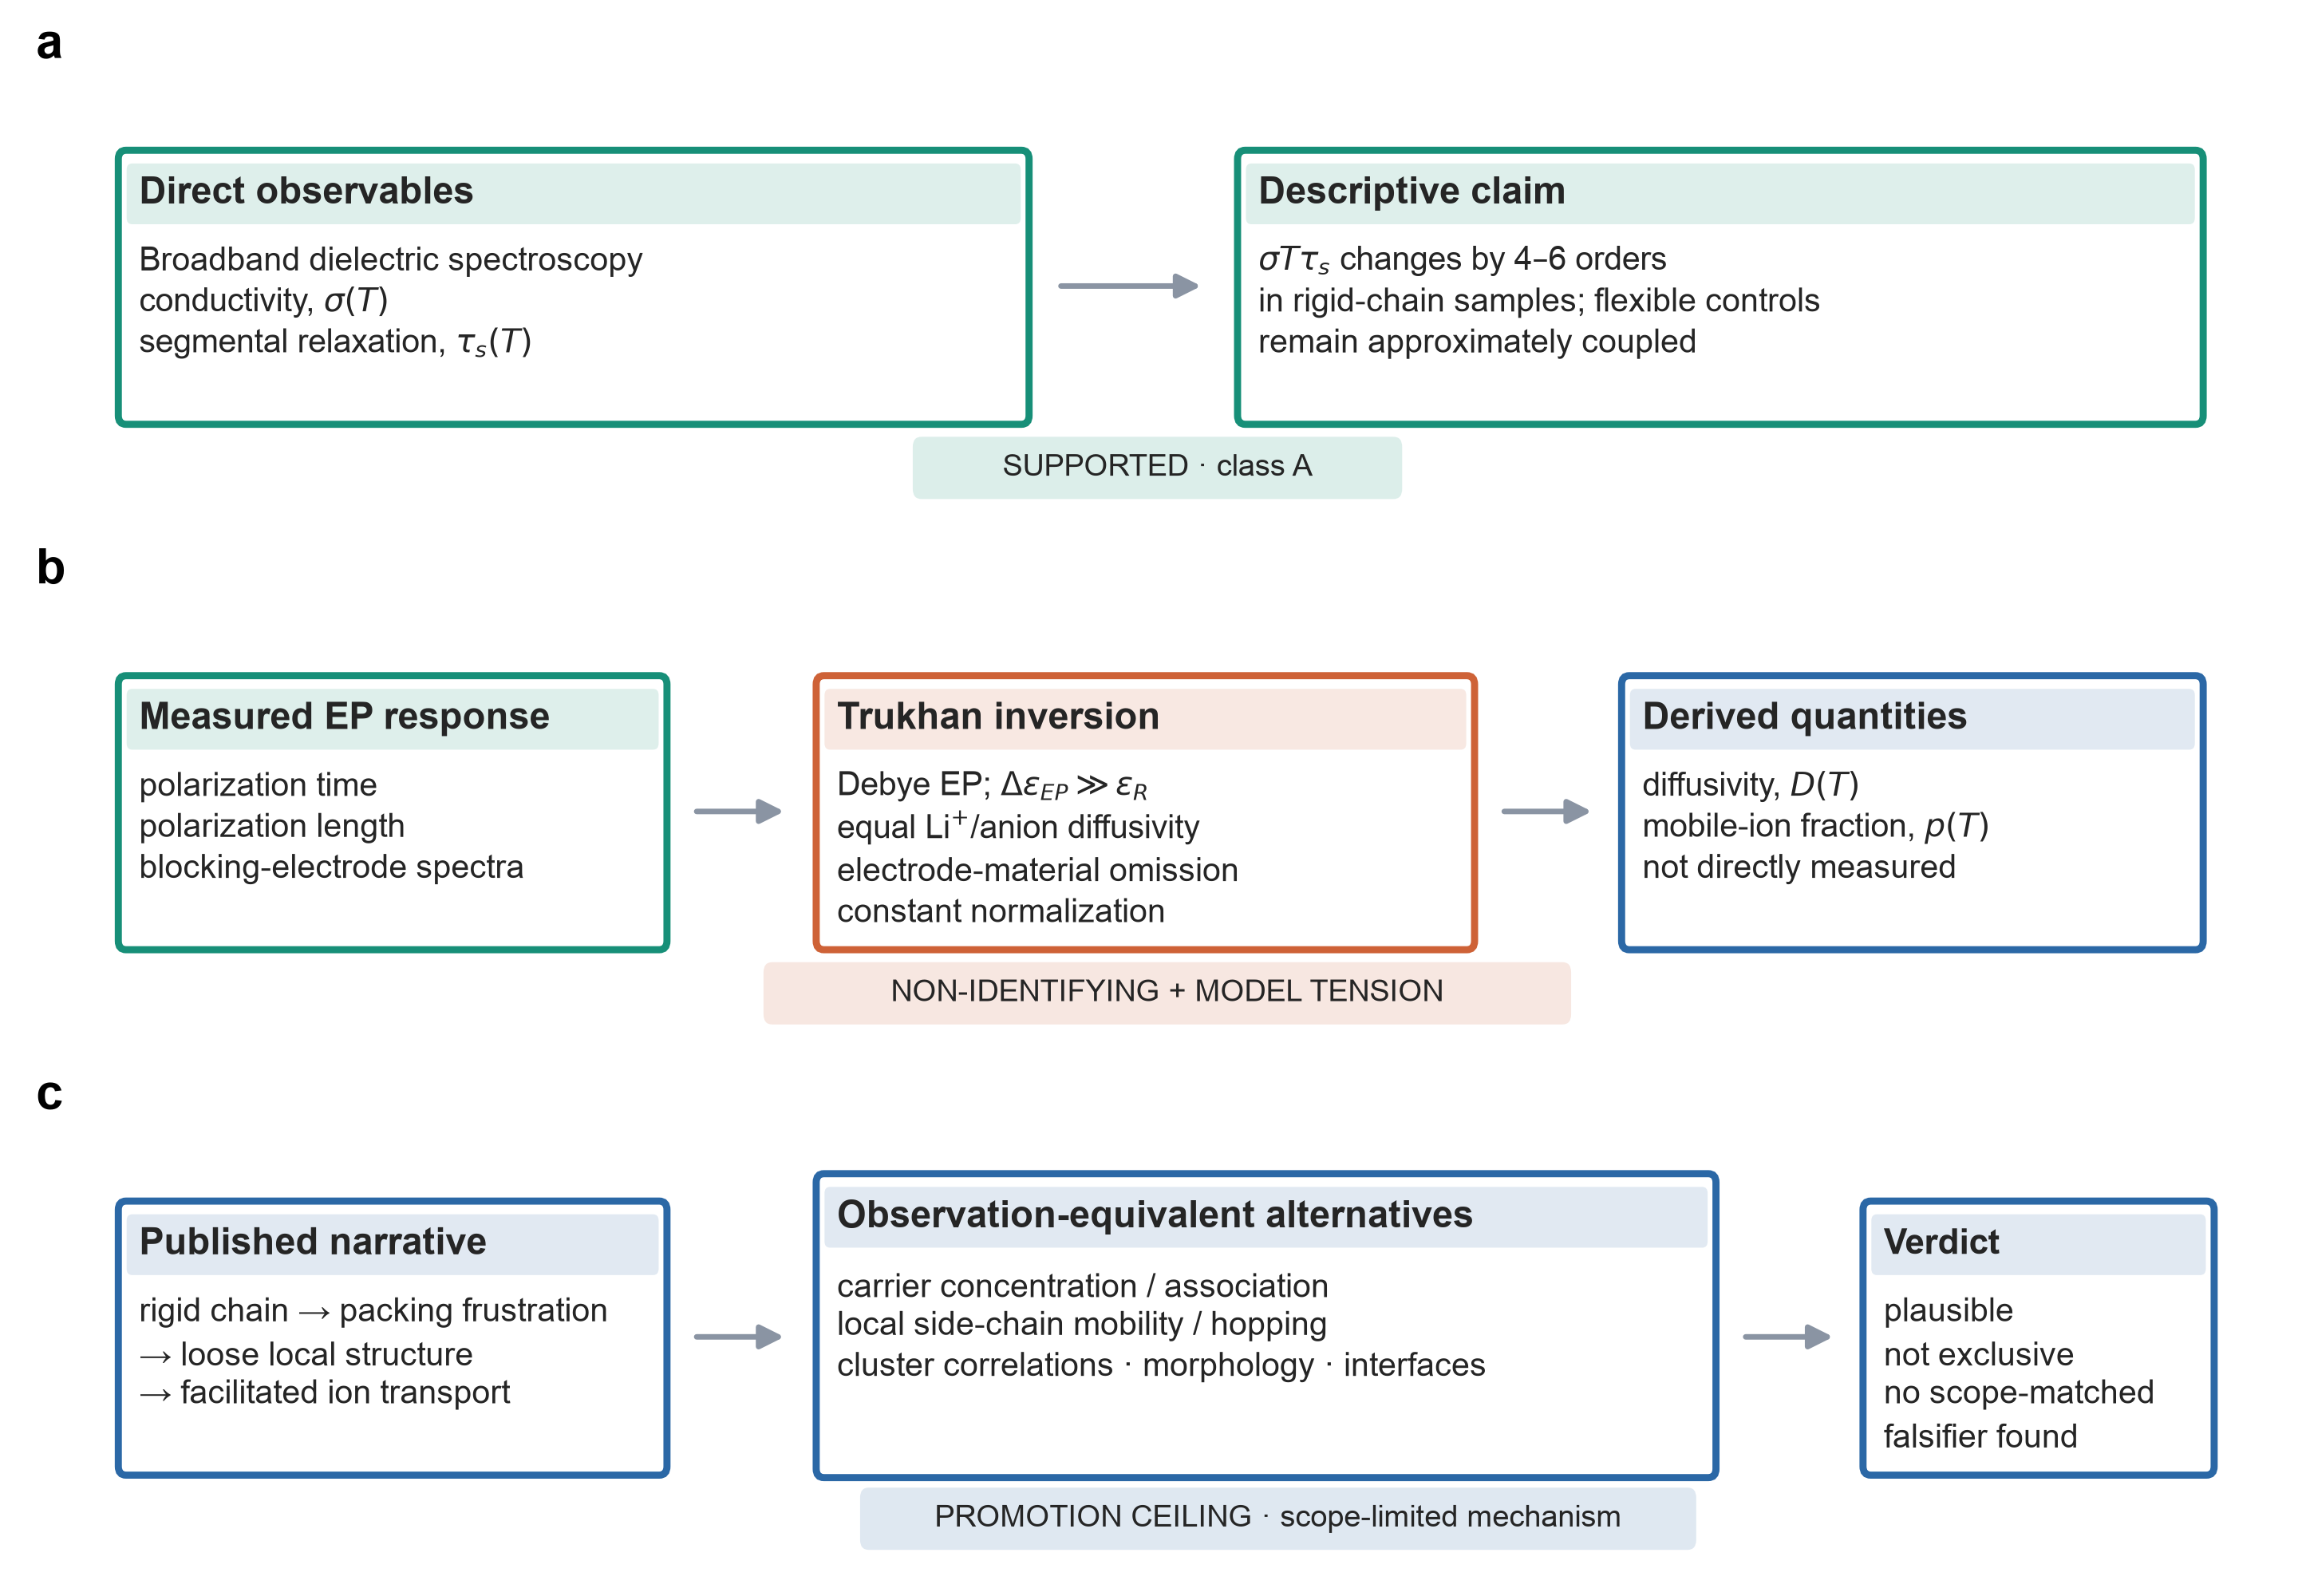
\includegraphics[width=0.96\textwidth]{figures/fig4_wang2012_evidence_ladder.png}
\caption{\textbf{Evidence layers in the polymer-electrolyte case.} \textbf{a,} Broadband dielectric spectroscopy directly supports the reported conductivity--segmental-relaxation departure in the named materials. \textbf{b,} Diffusivity and mobile-ion fraction are inverse-model outputs whose interpretation depends on electrode-polarization assumptions. \textbf{c,} Packing frustration is consistent with the observation but is not uniquely selected over alternative carrier, mobility, correlation or morphology pathways. No synthetic or digitized numerical data are shown.}
\label{fig:polymer}
\end{figure*}

The current evidence ceiling is therefore a source-grounded mechanism audit. The constrained model $M_0$ and free-slope model $M_1$ have been implemented with an errors-in-variables objective and tested on synthetic data. A curve-level empirical comparison has not been run because the public record available to this project does not contain raw $\sigma(T)$ and $\tau_s(T)$ values, fit covariance or an exact numerical definition of the fitting window.

\placeholder{Obtain or legally digitize the Wang curves, freeze temperature windows and digitization uncertainty, and compare $M_0$, a free-slope $M_1$ and a preregistered segmented $M_2$ by held-out conductivity prediction. Report each material separately; the published sequence of coupling exponents does not justify a rigid-versus-flexible binary.}

\subsection{Negative transference is a prospective closure case, not a completed result}

The planned deep polymer case asks when immobilizing anions, lowering anion self-motion or obtaining a high diffusion-based estimate licenses a claim about the sign and magnitude of the true lithium transference number. That inference depends on the reference frame and on Onsager cross-correlations, ion pairing and clustering, chain length and concentration. Later measurements in polyelectrolyte solutions report ion-correlation effects and negative lithium transference\cite{Bergstrom2023}; these data are scientifically valuable precisely because they can adjudicate a pre-outcome claim, but they must not be allowed to shape that claim retrospectively.

The preregistered case will therefore freeze a pre-outcome mechanism library and certificate before any outcome-dependent analysis. A formal countermodel will test whether the sign is determined while cross-correlations are unconstrained. Numerical/domain review will test physical admissibility. An independent reviewer will compare the theorem to the natural-language certificate. Only after these gates pass will the later measurement and associated public data be opened for mechanism-concordance analysis.

\placeholder{Insert the immutable RP execution receipt, formal theorem, independent semantic-fidelity review, numerical admissibility report and outcome-separated Dryad adjudication. Until all five artifacts exist, do not state that the workflow predicted negative transference or discovered its physical mechanism.}

\subsection{Three failure modes require three different closure observations}

Figure~\ref{fig:matrix} summarizes the evidence state. NASICON exhibits structural non-identifiability because a scalar barrier summary discards event-network organization. EIS/\nleis{} exhibits practical non-identifiability because finite noisy spectra and a flexible circuit leave a broad allocation set despite low held-out error. The polymer audit exhibits specification non-identifiability because a measured product and model-mediated inversion do not identify which physical factor changed. These are not three instances of one physical mechanism; they are three locations at which a many-to-one inference must be interrupted.

The matrix also prevents a common reporting error. A failed quantitative gate is a completed result, whereas an unperformed fidelity or empirical-closure gate is missing evidence. The former should be retained; the latter should remain a placeholder.

\begin{figure*}[t]
\centering
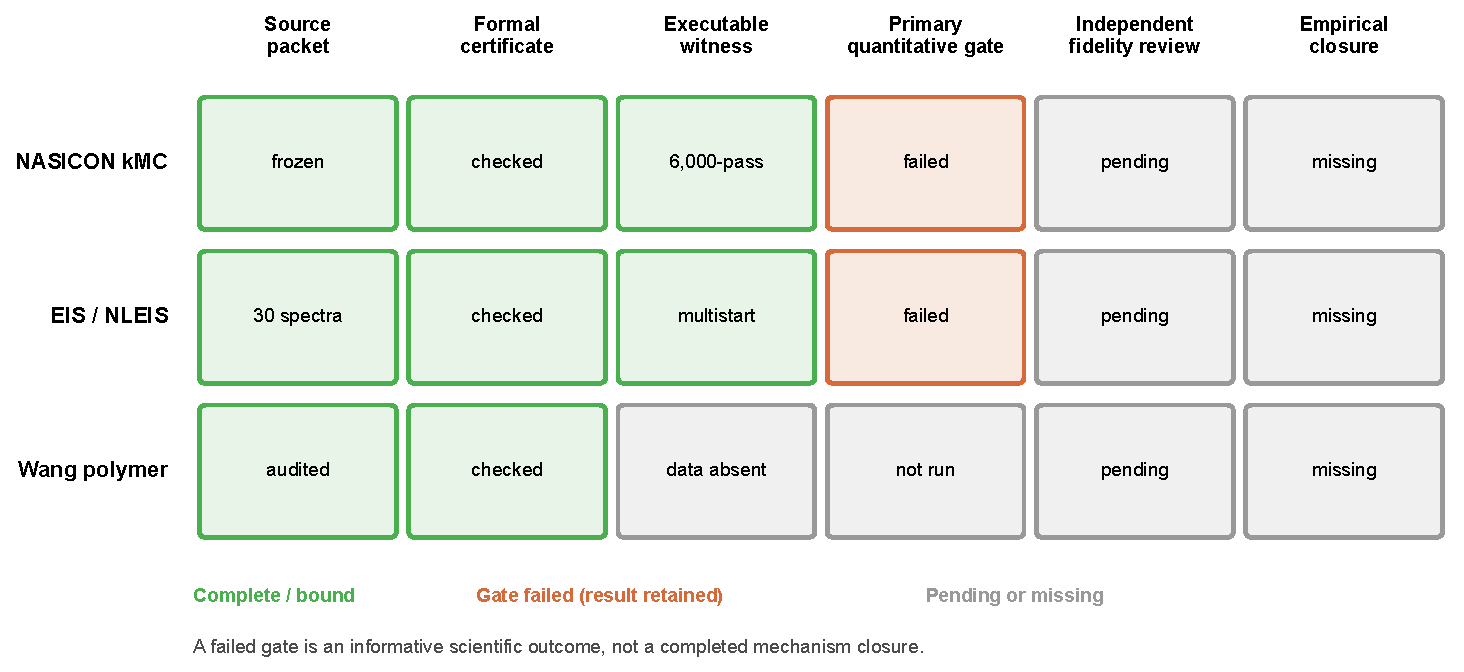
\includegraphics[width=0.98\textwidth]{figures/fig5_evidence_matrix.pdf}
\caption{\textbf{Claim--evidence matrix for the current draft.} Green indicates an available evidence layer, red a completed primary gate that failed, amber a pending review and grey a missing closure layer. A failed gate is informative and remains part of the evidence record; it is not equivalent to empirical closure. The three-case headline is withheld while fidelity and closure cells remain incomplete.}
\label{fig:matrix}
\end{figure*}

\begin{table*}[t]
\caption{Current claim ceilings and the experiments required for promotion.}\label{tab:roadmap}
\centering
\small
\begin{tabular}{>{\raggedright\arraybackslash}p{0.14\textwidth}>{\raggedright\arraybackslash}p{0.25\textwidth}>{\raggedright\arraybackslash}p{0.25\textwidth}>{\raggedright\arraybackslash}p{0.27\textwidth}}
\toprule
Case & Current defensible claim & Prohibited promotion & Required closure \\
\midrule
NASICON & Bounded counterexample and failed ordering promotion inside a pinned fitted \kmc{} model & General law or experimental pellet conductivity & Converged independent trajectories, event-network mediator and matched-temperature impedance \\
EIS/\nleis{} & Held-out predictive adequacy can coexist with weak allocation contraction in a fixed circuit study & Universal claim that \nleis{} is uninformative or that an electrode mechanism is false & Model-family robustness, calibrated uncertainty and independent electrode constraints \\
Wang polymer & Reported values reject a composite constant-$p$/constant-$H$/single-timescale null & Unique diffusion decoupling or packing mechanism & Raw/digitized curves, frozen windows and errors-in-variables out-of-sample comparison \\
Negative transference & Prospective protocol only & Claim of prediction, discovery or physical proof & Temporal seal, fidelity review, admissible witness and outcome-separated empirical adjudication \\
\bottomrule
\end{tabular}
\end{table*}

\section{Discussion}

Mechanism identification requires more than a successful forward prediction. It requires showing that plausible alternatives do not survive the admitted observations, or obtaining an additional observable that separates them. The three cases show how this requirement fails in different ways. A mean local descriptor is not an event network; a low-error whole-cell fit is not a stable electrode decomposition; and a conductivity trend is not a unique factorization into carriers, self-motion and collective correlations.

Formal verification is useful here because it forces quantifiers and premises into view. It can establish that a claimed invariant follows from a conjunction, or that two admissible assignments share an observable while differing in the target. This prevents a descriptive result from being silently promoted into a unique mechanism. Yet the same precision exposes the boundary of proof. If the formalization omits a reference frame, encodes the wrong observable or admits a physically impossible witness, kernel correctness does not rescue the scientific inference. Certificate provenance, independent fidelity review and domain admissibility are therefore co-equal with execution.

The failed NASICON and \nleis{} gates are not negative demonstrations of the technologies. NASICON \kmc{} remains capable of connecting migration landscapes to long-time transport, and second-harmonic impedance adds a parity channel absent from linear EIS. Our results instead constrain the claim that could be promoted from the selected data and protocol. Failure-preserving reporting is important because repeatedly changing convergence windows, circuits or thresholds until a mechanism appears identified would erase the evidentiary content of the prospective test.

The strongest future version of this study will close the loop experimentally. For NASICON, network-resolved diagnostics and matched samples must link the within-model counterexample to a material observable. For impedance, an independent electrode constraint must test whether numerical contraction corresponds to physical attribution. For polymers, species-resolved diffusion, electrophoretic or concentration-cell measurements, thermodynamic factors, spectroscopy of ion populations and structural/packing observables must be acquired on matched samples and thermal histories. A preregistered negative-transference case can then test whether formal non-entailment correctly identifies the missing correlation-sensitive observation.

\placeholder{The final Discussion will compare completed closure yield, cost and false-promotion rate across the three cases. Add this synthesis only after the common publication gate is complete and a blinded domain expert has reviewed each mechanism set.}

\section{Methods}

\subsection{Scientific-claim certificate and evidence classes}

Each case is represented by a versioned certificate containing the natural-language claim; strength, modality and scope; declared and hidden assumptions; physical hypothesis set and competitors; observables and reference frame; evidence provenance and temporal cutoff; structured and numerical obligations; formal target and source-node mapping; fidelity status; verifier outputs; proposed discriminating observation; and empirical-closure status. Evidence is classified as direct/descriptive support, non-identification, model tension or scope-matched counterexample. A literature tension is not treated as a falsifier unless material, intervention, observable and decision rule match the declared scope.

\subsection{NASICON data and frozen \kmc{} analysis}

The NASICON inputs and model code are pinned to the public \texttt{NASICON\_KMC\_paper\_data} repository at commit \texttt{69eb10b7c52d}. The held-out audit selected a matched pair using the declared barrier summaries before examining late-time conductivity. The 6,000-pass amendment retained three prespecified seeds (104729, 130363 and 155921), the fitted model, temperature, convergence metric and directional rule. Six raw trajectory shards and logs were hash-recorded. Pairwise late-window medians and gate decisions were aggregated without deleting non-converged runs. The result schema, full contract hash and all shard hashes are distributed with the repository.

\subsection{EIS/\nleis{} public corpus and multistart fitting}

The 30 paired spectra are pinned to the MIT-licensed \texttt{2nd-NLEIS-manuscripts} release at commit \texttt{859a0c75a649}; the fitting toolbox is pinned to \texttt{nleis.py} commit \texttt{71e472023fbb}. Each condition used a fixed held-out-frequency split and common multistart seeds. The preregistered analysis separately assessed held-out prediction error and contraction of the electrode-allocation range. All 30 spectrum-level result shards, the aggregate JSON and a proof receipt for the sum/difference countermodel are retained. Full commit identifiers are recorded in the repository. The aggregate runtime was 15,956.7\,s.

\subsection{Polymer source audit and forward-model contract}

The Wang audit binds the primary article and supporting information by DOI and content hash but does not redistribute publisher PDFs. The source chain separates fitted $\sigma$ and $\tau_s$ from electrode-polarization-derived $D$ and $p$, and from the packing-frustration narrative. The prospective curve-level analysis compares a constrained slope $\beta=-1$ with a free slope in
\begin{equation}
 \log[\sigma(T)T]=\alpha+\beta\log\tau_s(T),\qquad \epsilon=1+\beta,
\end{equation}
using an errors-in-variables likelihood so that noisy $\tau_s$ is not naively placed on both sides of an ordinary regression. The primary decision requires improved leave-one-temperature-out conductivity prediction, an interval for $\epsilon$ excluding zero, a material-scale effect size and robustness to window, digitization and influential-point choices. The executable fitter has passed known-slope synthetic tests; no empirical fit is reported here.

\subsection{Formal verification and fidelity boundary}

Lean obligations are intentionally minimal. They establish conditional invariants, non-injectivity or explicit countermodels over the encoded quantities. Kernel receipts record tool version, source hash, theorem target and return status. A successful receipt establishes syntactic and logical correctness under the encoded premises. Scientific promotion additionally requires an independent semantic-fidelity review linking every theorem term to the certificate and a numerical/domain review of each witness. At the time of this draft, independent fidelity review is pending and is not inferred from kernel success.

\subsection{Reproducibility and failure preservation}

The public repository contains contracts, raw public inputs, raw trajectory or fit shards, aggregate results, plotting scripts, formal sources, receipts and SHA-256 provenance. Validators check file integrity and pinned upstream commits but do not silently rerun multi-hour analyses. A failed preregistered gate is versioned as a result. A changed formalization, threshold or dataset requires a new protocol version and cannot overwrite the original outcome.

\section*{Data availability}

The NASICON and EIS/\nleis{} public inputs, processed result shards, figures and provenance records used in this draft are organized in the accompanying GitHub repository. Publisher PDFs are not redistributed; DOI records and hashes identify the audited copies. The Wang curve-level analysis remains blocked by raw or legally digitized numerical curves and covariance information. The negative-transference outcome data will be referenced only after the pre-outcome package is frozen.

\section*{Code availability}

Contracts, execution and aggregation scripts, plotting code, formal Lean sources and integrity validators are available at \url{https://github.com/yicao-tri/ARC-Mechanism-Closure-NPJ}. The manuscript source is mirrored under \texttt{paper/overleaf/}. Environment pins and exact upstream commits are documented in the repository.

\section*{Acknowledgements}

\placeholder{Add funding, computational resources, domain reviewers and data-provider acknowledgements after the author list and review roles are finalized.}

\section*{Author contributions}

\placeholder{Replace with a CRediT contribution statement after co-author roles and independent fidelity-review responsibilities are agreed.}

\section*{Competing interests}

\placeholder{Confirm the complete competing-interests statement for all authors before submission.}

\bibliography{sn-bibliography}

\end{document}
